\documentclass[autodetect-engine,11pt,a4paper,ja=standard]{bxjsarticle}

% NOTE: bxjsarticle already loads geometry with its own defaults.
% Override only what you need via \geometry{...} to avoid option clashes.
\geometry{margin=18mm}
\usepackage{graphicx}
\usepackage{booktabs}
\usepackage{tabularx}
\usepackage{longtable}
\usepackage{enumitem}
\usepackage{hyperref}
\usepackage{fancyhdr}
\usepackage{lastpage}
\usepackage{pdfpages} % optional: include multi-page schematics PDF

% ===== Project metadata (edit here) =====
\newcommand{\BoardName}{blackpulse\_esc\_v1.0}
\newcommand{\BoardSubtitle}{三相BLDCモーター用ESC基板}
\newcommand{\DocTitle}{データシート}
\newcommand{\DocRevision}{version 1.0}
\newcommand{\DocDate}{\today}

% ===== Cover page (datasheet-like) =====
\newcommand{\MakeCover}{%
	\begin{titlepage}
		\thispagestyle{empty}
		\noindent\rule{\linewidth}{0.8pt}\par
		\vspace{3mm}
		\noindent
		\begin{tabularx}{\linewidth}{@{}Xr@{}}
			{\normalsize （基板データシート）} & {\LARGE\bfseries \BoardName}\\
		\end{tabularx}\par
		\begin{tabularx}{\linewidth}{@{}Xr@{}}
			~ &
			
\includegraphics[height=10mm]{figures/logo1.jpg}
			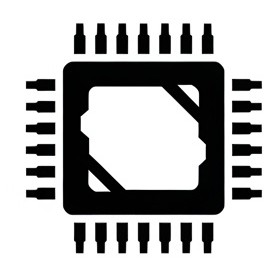
\includegraphics[height=10mm]{figures/logo2.jpg}
			
\includegraphics[height=10mm]{figures/logo3.jpg}
		\end{tabularx}\par
		

		\vspace{3mm}
		\begin{center}
			{\Large\bfseries \BoardSubtitle}\par
			\vspace{2mm}
			{\normalsize 製品仕様}\par
		\end{center}

		\vspace{2mm}
		\noindent\rule{\linewidth}{0.4pt}\par
		% \vspace{mm}

		\begin{minipage}[t]{0.50\linewidth}
			\vspace{2mm}
			{\bfseries 特長}\par
			\vspace{1mm}
			\begin{itemize}
				\item 50 x 50 mm(4層)のコンパクトな基板サイズ
				\item xt30による電源供給
				\item Hブリッジを6セット搭載し，2個の三相BLDCモーターを同時に制御可能
				\item ??Aの高い連続電流に対応（要確認）
				\item Vccは16-24Vの入力電圧に対応
				\item I2C/SPIによりセンサーの値を取得可能．
				\item encoder / hole sensorの入力に対応
				\item CAN(FD)を搭載しており，外部との高速な通信が可能
				\item プログラマブルLEDを搭載
				\item トグルスイッチを搭載しており，モード切替などに利用可能
				\item MCUにSTM32G431CBU6を搭載
				\item ゲートドライバにL6389EDTRを搭載し，回路の簡略化を実現
				\item ピンヘッダをショートさせることで，CANの終端抵抗のオンオフが可能
				\item 温度センサを搭載しており，過熱を防止可能
				\item パワー回路と制御回路のGNDの接点を一か所にすることにより，ノイズの低減を実現
			\end{itemize}
			\vspace{4mm}
			{\bfseries 文書情報}\par
			\vspace{1mm}
			\begin{tabularx}{\linewidth}{@{}lX@{}}
				リビジョン & \DocRevision \\
				作成日 & \DocDate \\
			\end{tabularx}
		\end{minipage}
		\hfill
		\begin{minipage}[t]{0.45\linewidth}

			\vspace{4mm}
			\begin{center}
				{\bfseries 製品写真}\par
				\vspace{2mm}
				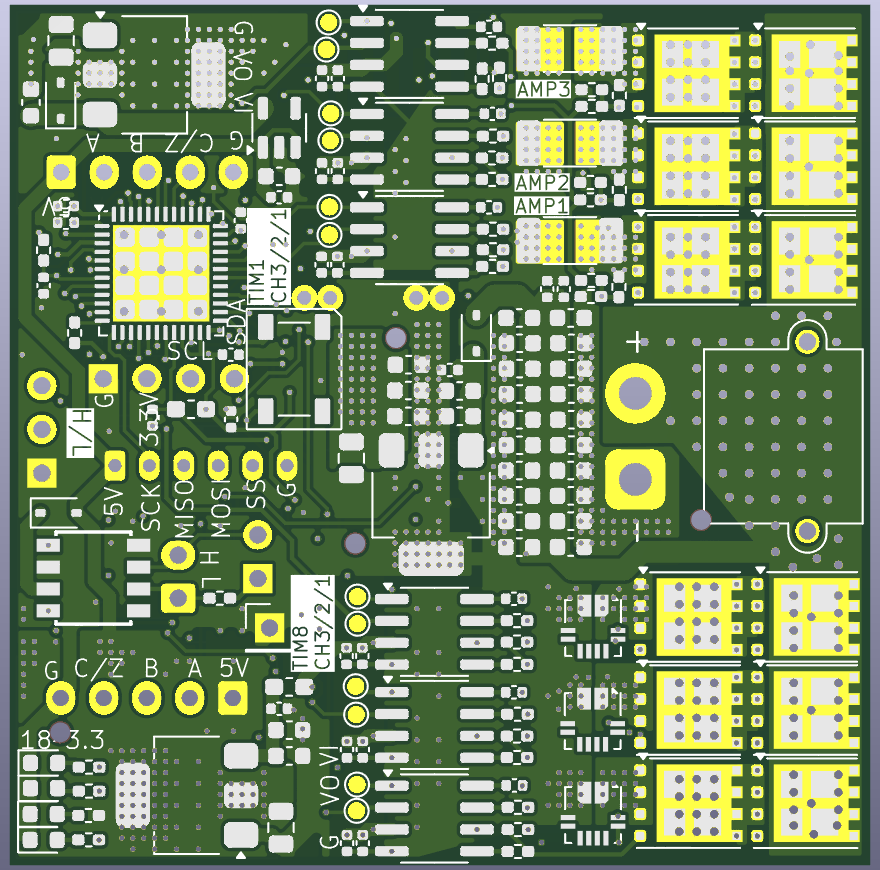
\includegraphics[width=0.8\linewidth]{figures/product_photo.png}
				% \fbox{\parbox{0.95\linewidth}{\vspace{22mm}\centering 製品写真（figures/product\_photo.* を配置）\vspace{22mm}}}
			\end{center}
			{\bfseries STM32G431CBU6の概要}\par
			\vspace{1mm}
			FPU/CORDICを用いた，高速な浮動小数点演算，FMACを用いたHWフィルタリングにより，20kHz以上の高い制御周期でのFOC制御を可能とする．また、ホールセンサーやエンコーダー入力に対応し，幅広いモーターに対応可能．通信インターフェースはCAN(FD)やSPIをサポートしている．
			\\
		\end{minipage}

		\vfill
		\noindent\rule{\linewidth}{0.8pt}\par
		\vspace{2mm}
		\footnotesize
		% \noindent \DocRevision\hfill \thepage
	\end{titlepage}
}

\hypersetup{
	colorlinks=true,
	linkcolor=black,
	urlcolor=black,
	citecolor=black,
	pdftitle={\BoardName\ \DocTitle},
}

% ===== Header / Footer (lines top & bottom on every page) =====
\pagestyle{fancy}
\fancyhf{}

% Header
\fancyhead[L]{\BoardName}
\fancyhead[C]{\DocTitle}
\fancyhead[R]{\DocRevision\;\;\DocDate}

% Footer
\fancyfoot[L]{%
	
\includegraphics[height=6mm]{figures/logo1.jpg}
}
\fancyfoot[R]{%
	\thepage\,/\,\pageref*{LastPage}
}

\setlength{\headheight}{18pt}

% footer画像用に少し余裕を増やす
\setlength{\footskip}{24pt}

\renewcommand{\headrulewidth}{0.6pt}
\renewcommand{\footrulewidth}{0.6pt}

\setlength{\parindent}{0pt}
\setlist[itemize]{noitemsep, topsep=4pt}
\setlist[enumerate]{noitemsep, topsep=4pt}

\begin{document}
\MakeCover

\pagestyle{fancy}
\thispagestyle{fancy}

% \vspace{-2mm}
% \begin{tabularx}{\linewidth}{@{}lX@{}}
% \toprule
% 項目 & 内容 \\
% \midrule
% 対象基板 & \BoardName \\
% リビジョン & \DocRevision \\
% 作成日 & \DocDate \\
% 備考 & （ここに用途や対象システムなどを1行） \\
% \bottomrule
% \end{tabularx}

\tableofcontents
\newpage

\section{概要（Description）}
\subsection{目的・用途}
この基板は，2個の三相BLDCモーターを制御することを目的とした基板であり，
入力電圧(Vcc)は16-24V，最大連続電流は??Aに対応している．
電流検知機能，温度監視機能，センサーポート/通信用ポートを備えており，エンドノードとしての利用を想定している．
CAN(FD)の終端抵抗のオンオフも可能である．


\subsection{主要仕様}
% 数字がまだ未確定なら「TBD」でOK
\begin{tabularx}{\linewidth}{@{}lX@{}}
\toprule
項目 & 値 \\
\midrule
入力電圧範囲 & 16-24V \\
最大連続電流 & ??A \\
MCU/制御方式 & STM32G431CBU6 / FOC \\
通信IF & CAN(FD), UART, I2C, SPI \\
センサー & ADC, Encoder/Hole sensor \\
保護機能 & 過電流保護, 過温度保護 \\
\bottomrule
\end{tabularx}

\newpage
\section{ポート設定（Ports / Pinout）}
% 「コネクタ単位」でテーブルを分けるのがおすすめです。
ポート一覧の概要図を図\ref{fig:pinout_overview}に示す。
デバッグ用のGNDピン(J3)は省いている．
\begin{figure}[htbp]
	\centering
	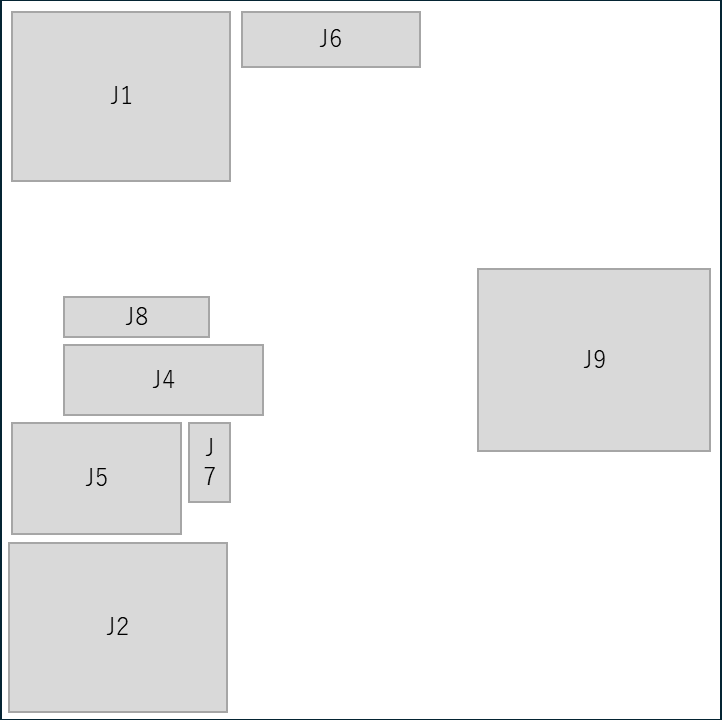
\includegraphics[width=0.6\linewidth]{figures/port.png}
	% \fbox{\parbox{0.95\linewidth}{\vspace{18mm}\centering ポート配置図（figures/pinout\_overview.* を配置）\vspace{18mm}}}
	\caption{ポート配置の概要図}
	\label{fig:pinout_overview}
\end{figure}
\subsection{コネクタ一覧}
コネクタの種類と役割の一覧を以下に示す。\\
\\
\begin{tabularx}{\linewidth}{| @{}l| l| X@{}|}
% \toprule
\hline
名称 & コネクタ/部品 & 備考 \\
% \midrule
\hline
J1 & 1x5ピンヘッダ & センサーポート1 \\
J2 & 1x5ピンヘッダ & センサーポート2 \\
J3 & 1x1ピンヘッダ & デバッグ用GNDピン \\
J4 & 1x6ピンヘッダ & SPI用ポート \\
J5 & 1x2ピンヘッダ & CAN(FD)用ポート \\
J6 & 1x6ピンヘッダ & デバッグ用ポート \\
J7 & 1x2ピンヘッダ & 終端抵抗オンオフジャンパ \\
J8 & 1x4ピンヘッダ & I2C用ポート \\
J9 & XT30 & 電源入力 \\

% \bottomrule
\hline
\end{tabularx}

\subsection{ピンアサイン}
ピンアサイン一覧を以下の表に示す．
% longtableにしているので、行数が増えてもページまたぎできます。
\begin{longtable}{@{}l l l l p{0.48\linewidth}@{}}
\toprule
コネクタ & ピン & 信号名 & 方向 & 説明 \\
\midrule
\endfirsthead
\toprule
コネクタ & ピン & 信号名 & 方向 & 説明 \\
\midrule
\endhead
\midrule
\multicolumn{5}{r}{次ページへ続く}\\
\endfoot
\bottomrule
\endlastfoot

J1 & 1 & Vcc & o & 電源出力(5V) \\
~ & 2 & CH1 & i/o & encoder\_A / SPI1\_MISO \\
~ & 3 & CH2 & i/o & encoder\_B / SPI1\_MOSI \\
~ & 4 & CH3 & i/o & encoder\_Z / SPI1\_SCK \\
~ & 5 & GND & - & グランド \\
\midrule
J2 & 1 & Vcc & o & 電源出力(5V) \\
~ & 2 & CH1 & i/o & hole\_sensor\_1 / encoder\_A / \\
~ & 3 & CH2 & i/o & hole\_sensor\_2 / encoder\_B / \\
~ & 4 & CH3 & i/o & hole\_sensor\_3 / encoder\_Z / \\
~ & 5 & GND & - & グランド \\
\midrule
J3 & 1 & GND & - & グランド \\
\midrule
J4 & 1 & Vcc & o & 電源出力(5V) \\
~ & 2 & SCK & o & SPIクロック \\
~ & 3 & MISO & i & SPIマスタからの入力 \\
~ & 4 & MOSI & o & SPIマスタへの出力 \\
~ & 5 & CS & o & SPIチップセレクト \\
~ & 6 & GND & - & グランド \\
\midrule
J5 & 1 & CAN\_H & i/o & CANの高レベル信号 \\
~ & 2 & CAN\_L & i/o & CANの低レベル信号 \\
\midrule
J6 & 1 & Vcc & i & 電源入力(3.3V) \\
~ & 2 & SWDIO & i/o & SWDデータ \\
~ & 3 & SWCLK & i & SWDクロック \\
~ & 4 & GND & - & グランド \\
~ & 5 & TX & o & UART送信 \\
~ & 6 & RX & i & UART受信 \\
\midrule
J7 & 1 & CAN\_H & - & 終端抵抗オンオフ用ジャンパ \\
~ & 2 & CAN\_L\_R & - & 終端抵抗オンオフ用ジャンパ \\
\midrule
J8 & 1 & GND & - & グランド \\
~ & 2 & Vcc & o & 電源出力(3.3V) \\
~ & 3 & SCL & o & I2Cクロック \\
~ & 4 & SDA & o & I2Cデータ \\
\midrule
J9 & 1 & GND & - & グランド \\
~ & 2 & Vcc & i & 電源入力(16-24V) \\
\end{longtable}

\subsection{ポート設定（ソフトウェア）}
ソフトウェアでのMCUでのピン設定を図\ref{fig:pinout_software}と
以下の表に示す。
\begin{figure}[htbp]
	\centering
	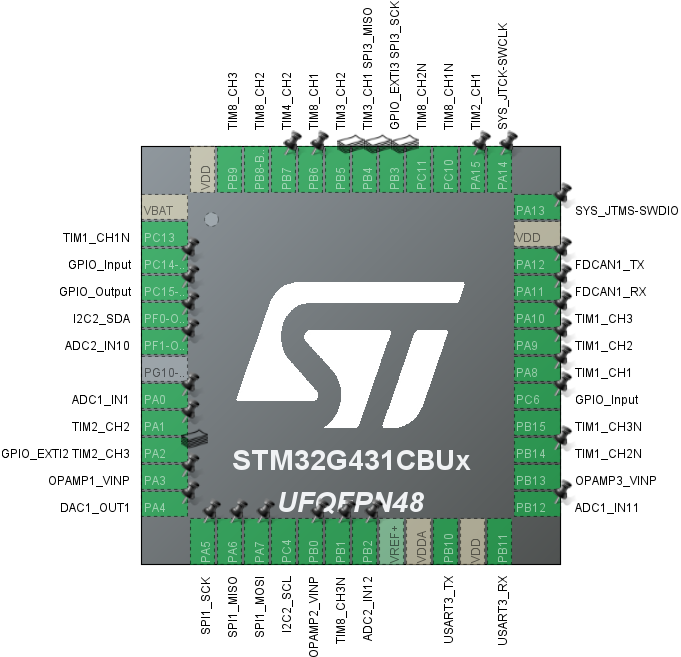
\includegraphics[width=0.8\linewidth]{figures/pins.png}
	% \fbox{\parbox{0.95\linewidth}{\vspace{18mm}\centering ピンアサイン図（figures/pinout\_detailed.* を配置）\vspace{18mm}}}
	\caption{MCUのピンアサイン図}
	\label{fig:pinout_software}
\end{figure}
% 例：STM32のピン設定や、タイマ/ADC/コンパレータの割り当て等
\begin{longtable}{@{}l l l l l p{0.48\linewidth}@{}}
\toprule
役割 & 信号名 & ピン番号 & 内部割り当て & 説明 \\
\midrule
\endfirsthead
% \textbf{ポート設定（ソフトウェア）} \\
\toprule
役割 & 信号名 & ピン番号 & 内部割り当て & 説明 \\
\midrule
\endhead
\midrule
% \multicolumn{5}{r}{次ページへ続く}\\
\endfoot
\bottomrule
\endlastfoot
% 6個の電源ピン，不使用ポート一個のみで，41個の信号ピンがある
NRST & NRST & PG10 & NRST & リセット入力 \\
\midrule % 6
PWM1 & CH1 & PA8 & TIM1\_CH1 & モーター1制御PWM出力U \\
~ & CH2 & PA9 & TIM1\_CH1 & モーター1制御PWM出力V \\
~ & CH3 & PA10 & TIM1\_CH1 & モーター1制御PWM出力W \\
~ & CH1N & PC13 & TIM1\_CH1 & モーター1制御PWM出力U(反転) \\
~ & CH2N & PB13 & TIM1\_CH1 & モーター1制御PWM出力V(反転) \\
~ & CH3N & PA15 & TIM1\_CH1 & モーター1制御PWM出力W(反転) \\
\midrule % 6(12)
PWM2 & CH1 & PB6 & TIM8\_CH1 & モーター2制御PWM出力U \\
~ & CH2 & PB8 & TIM8\_CH1 & モーター2制御PWM出力V \\
~ & CH3 & PB9 & TIM8\_CH1 & モーター2制御PWM出力W \\
~ & CH1N & PC10 & TIM8\_CH1 & モーター2制御PWM出力U(反転) \\
~ & CH2N & PC11 & TIM8\_CH1 & モーター2制御PWM出力V(反転) \\
~ & CH3N & PB1 & TIM8\_CH1 & モーター2制御PWM出力W(反転) \\
\midrule % 3(15)
電流検知1 & AMP1 & PA3 & OPAMP1\_VINP & W相の電流検知アンプ入力 \\
~ & AMP2 & PB0 & OPAMP2\_VINP & V相の電流検知アンプ入力 \\
~ & AMP3 & PB13 & OPAMP3\_VINP & U相の電流検知アンプ入力 \\
\midrule % 3(18)
電流検知2 & ADC1 & PB12 & ADC1\_IN11 & W相の電流検知ADC入力 \\
~ & ADC2 & PB2 & ADC2\_IN12 & V相の電流検知ADC入力 \\
~ & ADC3 & PF1 & ADC2\_IN10 & U相の電流検知ADC入力 \\
\midrule % 1(19)
温度センサ & ADC4 & PA0 & ADC1\_IN1 & 内部温度センサのADC入力 \\
\midrule % 3(22)
J1 & CH1 & PB3 & TIM3\_CH1 | SPI3\_MISO & センサー入力1\\
~ & CH2 & PB4 & TIM3\_CH2 | SPI3\_MOSI & センサー入力2\\
~ & CH3 & PB5 & EXIT13 | SPI3\_SCK & センサー入力3\\
\midrule % 3(25)
J2 & CH1 & PA15 & TIM2\_CH1 & センサー入力1\\
~ & CH2 & PA1 & TIM2\_CH2 & センサー入力2\\
~ & CH3 & PA2 & EXIT2 | TIM2\_CH3 & センサー入力3\\
\midrule % 4(29)
J4 & SCK & PA5 & SPI1\_SCK & SPIクロック \\
~ & MISO & PA6 & SPI1\_MISO & SPIマスタからの入力 \\
~ & MOSI & PA7 & SPI1\_MOSI & SPIマスタへの出力 \\
~ & CS & PC15 & SPI1\_NSS & SPIチップセレクト \\
\midrule % 2(31)
CAN & CAN\_TX & PA12 & FDCAN1\_TX & CAN送信 \\
~ & CAN\_RX & PA11 & FDCAN1\_RX & CAN受信 \\
\midrule % 6(37)
J6 & SWDIO & PA13 & SWDIO & SWDデータ \\
~ & SWCLK & PA14 & SWCLK & SWDクロック \\
~ & TX & PB10 & USART3\_TX & UART送信 \\
~ & RX & PB11 & USART3\_RX & UART受信 \\
\midrule % 2(39)
J8 & SCL & PC4 & I2C2\_SCL & I2Cクロック \\
~ & SDA & PF0 & I2C2\_SDA & I2Cデータ \\
\midrule % 1(40)
LED & DIO & PB7 & TIM4\_CH2 & DMAを使用し色指定 \\
\midrule % 1(41)
SW & Toggle & PC14 & GPIO\_input | EXIT14 & トグルスイッチ入力 \\
\end{longtable}

\section{機能説明（Functional Description）}
\subsection{システム構成}
システム構成を図\ref{fig:block_diagram}に示す。

\begin{figure}[htbp]
	\centering
	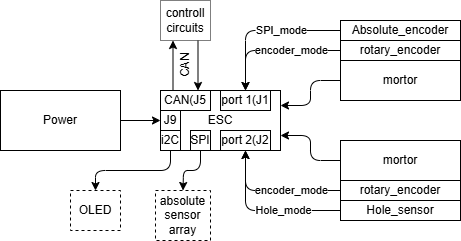
\includegraphics[width=0.8\linewidth]{figures/block_diagram.drawio.png}
	% \fbox{\parbox{0.95\linewidth}{\vspace{18mm}\centering ブロック図（figures/block\_diagram.* を配置）\vspace{18mm}}}
	\caption{システム構成（ブロック図）}
	\label{fig:block_diagram}
\end{figure}
\newpage
\subsection{電源系}
\begin{itemize}
	\item 入力保護：TBD
	\item レギュレータ：TBD
	\item 監視：TBD（UVLO/OVPなど）
\end{itemize}

\subsection{ゲート駆動・パワーステージ}
\begin{itemize}
	\item ハーフブリッジ：TBD
	\item ゲートドライバ：TBD
	\item 電流検出：TBD
	\item 逆起電力/位置推定：TBD（必要なら）
\end{itemize}

\subsection{保護機能}
\begin{itemize}
	\item 過電流：TBD
	\item 過温度：TBD
	\item 低電圧：TBD
\end{itemize}

\section{回路図（Schematics）}
% KiCadからPDF出力したものを figures/ に置くのが運用しやすいです。
% - 単ページPDF/PNGなら \includegraphics
% - 複数ページPDFなら \includepdf（pdfpages）

\subsection{全体回路図（1枚の場合）}
\begin{figure}[h]
	\centering
	% \includegraphics[width=\linewidth]{figures/schematic_overview.pdf}
	\fbox{\parbox{0.95\linewidth}{\vspace{22mm}\centering 回路図（figures/schematic\_overview.* を配置）\vspace{22mm}}}
	\caption{回路図（概要）}
\end{figure}

\subsection{回路図（複数ページPDFの場合）}
% 例：figures/schematics.pdf に全ページをまとめて出力した場合
% \includepdf[pages=-,pagecommand={\thispagestyle{fancy}}]{figures/schematics.pdf}

\section{改訂履歴（Revision History）}
\begin{tabularx}{\linewidth}{@{}l l X@{}}
\toprule
日付 & Rev & 変更内容 \\
\midrule
\DocDate & \DocRevision & 初版（テンプレ作成） \\
\bottomrule
\end{tabularx}

\end{document}
